In this chapter we introduce a technique for improving the scalability of safety validation algorithms for multi-agent systems. We first describe the problem of exponential growth of states and disturbances with respect to the number of adversarial entities. We then show how multi-agent safety validation problems can be decomposed into subproblems each involving the system interacting with a subset of the adversaries. The solution to these subproblems can be recombined using an attention network and a base network to correct for multi-agent interactions. We demonstrate the efficacy of scene decomposition by approximating the distribution over failures of a multi-agent gridworld and T-intersection scenario. 

\section{Motivation}

%todo:cite airspace density commment below
Many of the most exciting use cases for autonomy require the system to interact with large number of other human and non-human agents. An autonomous driving policy must reason about a potentially large number other vehicles, pedestrians, cyclists, and traffic control systems, each with a wide variety of possible behaviors. Similarly, autonomous aircraft will soon have to navigate and avoid collisions in an increasingly dense airspace.

Many of the challenges for safety validation are exacerbated when the environment contains multiple interacting agents. The dimensionality of both the disturbance and state space grows with each new agent in the environment. The search over disturbance trajectories, state-dependent policies, or the state space itself can quickly become intractable. As a probability, failures may be more or less likely with more agents, but the fraction of the disturbance trajectory space that leads to a failure will likely decrease due to the dramatic increase in the size of the disturbance trajectory space. 

As an example, consider the $5 \times 5$ adversarial gridworld problem depicted in \cref{fig:ch6_fullg} where an ego agent (blue) tries to avoid two adversarial agents (orange and red).  Each agent has a 2D position and four possible actions so the state space and disturbance space both grow exponentially with the number of agents. In this case, a failure occurs when all agents overlap on the same state, so failures become less likely with the number agents. Value iteration is tractable on this problem with two adversaries (which is why we include it as a test case), but becomes very challenging with \num{3} agents and completely intractable with more.

The curse of dimensionality is a well known problem in multi-agent systems and is often solved by decomposing the problem into simpler problems that are tractable and then recombining the solutions. In this chapter we develop a technique for decomposing and recombining safety validation problems. The basic idea is to identify a natural decomposition of the state space that reduces the full problem into a set of subproblems that can be solved individually. For example, the gridworld with two adversaries can be decomposed into two gridworlds, each with a single adversary (as shown in \cref{fig:ch6_subg1,fig:ch6_subg2}). Then, to solve the full problem we learn how to combine the subproblem solutions instead of solving the problem from scratch. The solution to the full problem may not be a simple combination of the subproblem solutions so we simultaneously learn a correction factor. 

For this procedure to be successful, however, we need the subproblem solutions to confer some benefit to the solution of the full problem. In the case of the gridworld example, the subproblem solutions will suggest that it is beneficial to move toward the ego to cause failure. This insight will likely aid the adversary when solving the full problem.

In the next section we formalize the decomposition and highlight some potential efficiencies. We then demonstrate that combining the subproblems can be cast as a transfer learning problem and we apply a known transfer learning algorithm to solve it. 


\begin{figure*}
    \centering
    \begin{subfigure}[b]{0.25\textwidth}
        \centering
        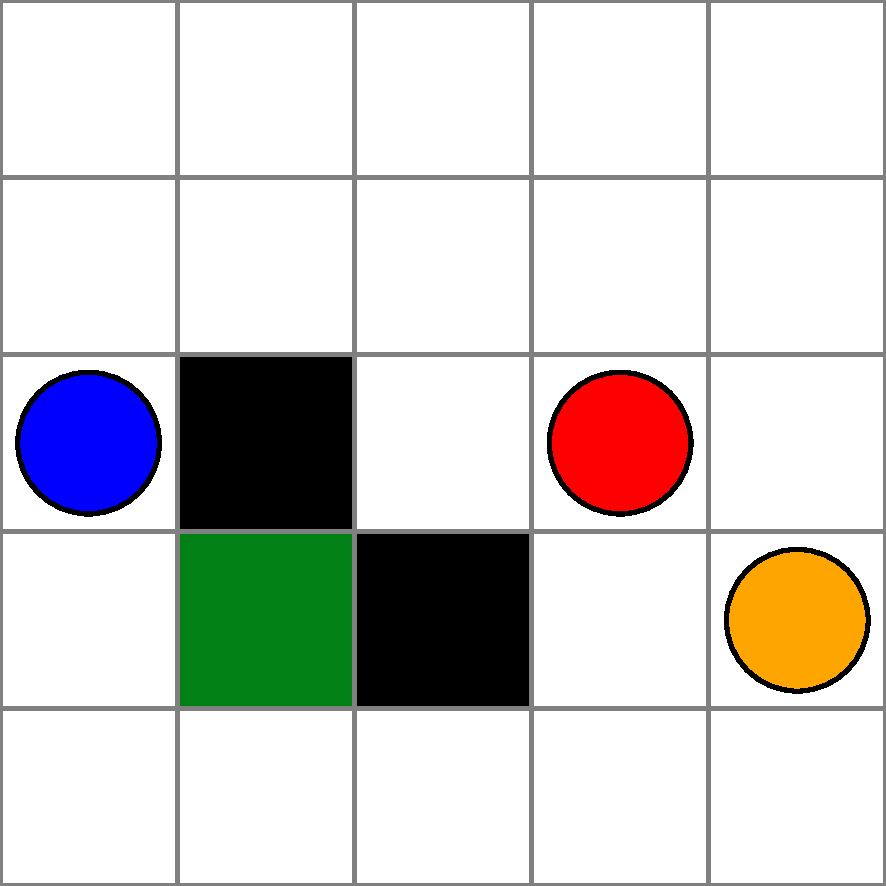
\includegraphics[width=\textwidth]{figures/scene_decomposition/g.pdf}
        \caption{Full problem.}
        \label{fig:ch6_fullg}
    \end{subfigure}
    \hfill
    \begin{subfigure}[b]{0.25\textwidth}
        \centering
        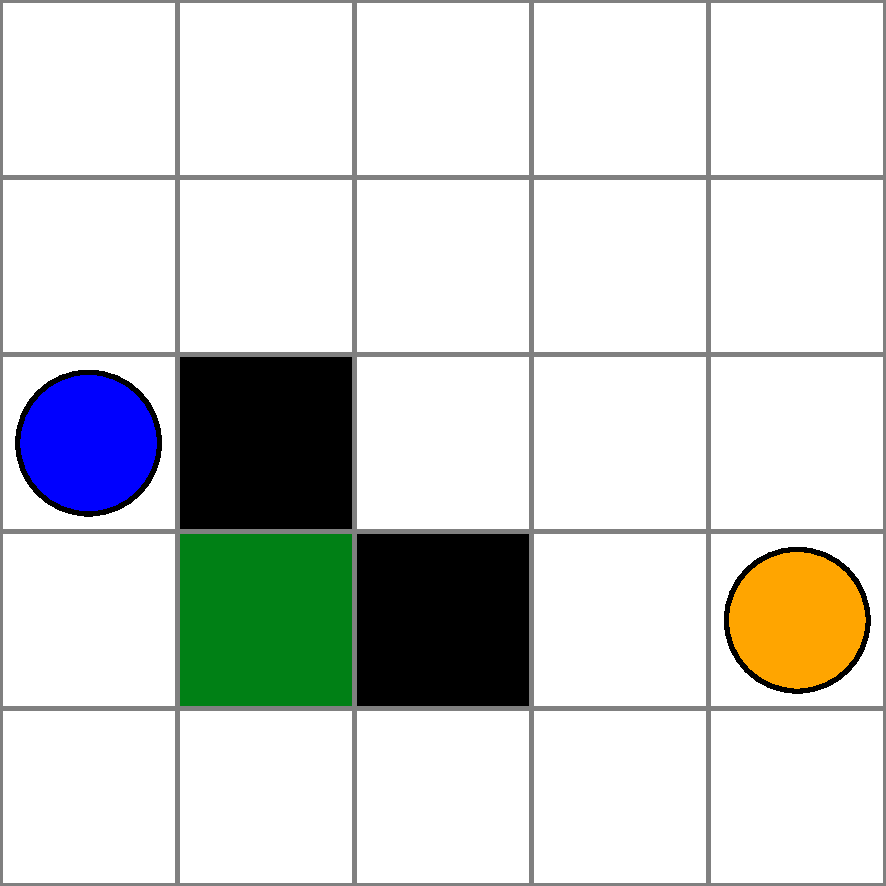
\includegraphics[width=\textwidth]{figures/scene_decomposition/g_sub1.pdf}
        \caption{Subproblem 1}
        \label{fig:ch6_subg1}
    \end{subfigure}
    \hfill
    \begin{subfigure}[b]{0.25\textwidth}
        \centering
        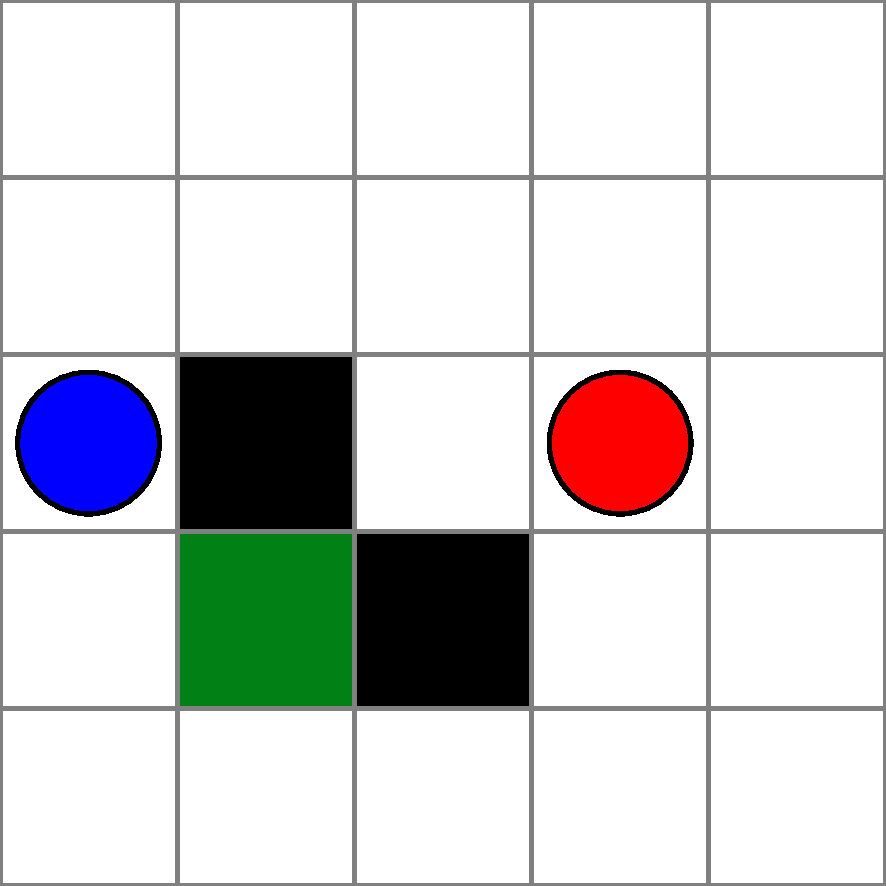
\includegraphics[width=\textwidth]{figures/scene_decomposition/g_sub2.pdf}
        \caption{Subproblem 2.}
        \label{fig:ch6_subg2}
    \end{subfigure}
    \caption{Example decomposition of the gridworld with two adversaries.}
    \label{fig:adv_gridworld_decomp}
\end{figure*}

\section{Decomposition and Fusion}
In this section we describe the process of problem decomposition and identify situations where subproblems are identical. We then introduce the attend, adapt, and transfer algorithm that automatically learns how to combine the subproblem solutions while learning a correction factor. 

\subsection{Problem Decomposition}
The goal of state-space decomposition is to identify a set of subspaces that each represent a similar, but smaller, version of the full problem. We denote the state space of the $i$th subproblem $S^{(i)}$ and the disturbance space $X^{(i)}$. The state $s^{(i)} \in S^{(i)}$ contains the components of $s$ that are associate with the $i$th subproblem and similarly for the disturbance $x^{(i)}$. A crucial constraint on the choice of decomposition is the ability to simulate transitions of the subproblems
\begin{equation}
    s_{t+1}^{(i)} \sim P( s^{(i)} \mid s_t^{(i)}, x_t^{(i)} ) \text{.}
\end{equation}

In the gridworld example, if we choose a decomposition where the state space consists only of the horizontal component of each agent, it is not clear how we would choose a transition model that is faithful to the original problem. Instead, if we choose a decomposition where the state space is the position of the ego and one adversary, and the disturbance space is the disturbance space of that adversary then we have reduced the problem a single-adversary gridworld which we know how to simulate. Indeed, in multi-agent problems a natural decomposition usually consists of the state spaces from a subset of of the agents. 

In 

\subsection{Solution Fusion}

\begin{equation}
\hat{Q}(s) = w_0(s) \hat{Q}_{\rm base}(s) + \sum_{i=1}^k w_i(s) g_x^{(i)}(\hat{Q}_i(g_s^{(i)}(s)))
\end{equation}

\begin{figure}[!t]
\centering
% TikZ diagram for black-box safety validation problem formulation.
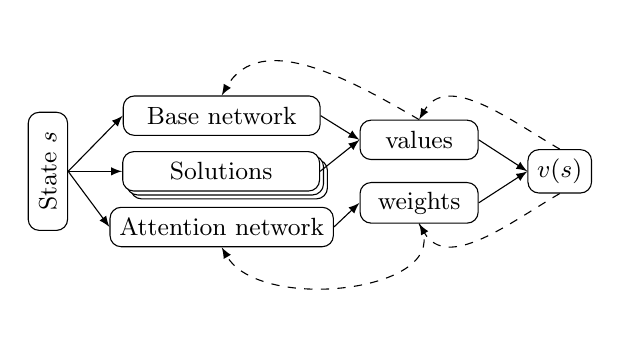
\begin{tikzpicture}
    \tikzstyle{every node}=[font=\small, align=center]
    \tikzset{
        n/.style={draw, rounded corners, minimum height=0.5cm, minimum width = 1.5cm},
        n2/.style={n, minimum width=2.5cm}
        }
    
    %state 
    \node (state) [n, rotate=90] {\small State $s$};
    
    %base network
    \node (base) [n2, above right of=state, xshift=1.5cm] {Base network};
    
    %Solutions
    \node (solutionsback1) [n2, right of=state, xshift=1.3cm, yshift=-0.1cm] {};
    \node (solutionsback2) [n2, fill=white, right of=state, xshift=1.25cm, yshift=-0.05cm] {};
    \node (solutions) [n2, fill=white, right of=state, xshift=1.2cm] {Solutions};
    
    %weights
    \node (attn) [n2, below right of=state, xshift=1.5cm] {Attention network};
    

    \node (values) [n, below right of=base, xshift=1.8cm, yshift = 0.4cm] {values};
    
     \node (weights) [n, above right of=attn, xshift=1.8cm, yshift = -0.4cm] {weights};
     
     \node (pfail) [n, minimum width = 0.5cm, right of=state, xshift=5.5cm] {$v(s)$};
    

    \draw[-latex] (state.south) -- (base.west);
    \draw[-latex] (state.south) -- (solutions.west);
    \draw[-latex] (state.south) -- (attn.west);
    
    \draw[-latex] (base.east) -- (values.west);
    \draw[-latex] (solutions.east) -- (values.west);
    \draw[-latex] (attn.east) -- (weights.west);
    
    \draw[-latex] (weights.east) -- (pfail.west);
    \draw[-latex] (values.east) -- (pfail.west);
    
    
    % backprop
    
    \draw [dashed, -latex] (weights.south) to [out=-1500,in=-60] (attn.south);
    \draw [dashed, -latex] (pfail.south) to [out=-150,in=-60] (weights.south);
    \draw [dashed, -latex] (values.north) to [out=150,in=60] (base.north);
    \draw [dashed, -latex] (pfail.north) to [out=150,in=60] (values.north);
\end{tikzpicture}
\caption{The A2T network. }
\label{fig:A2T_Network}
\vskip -0.5cm
\end{figure}



\section{Experiments}

\section{Adversarial Gridworld Example}

\begin{figure}
        \centering
        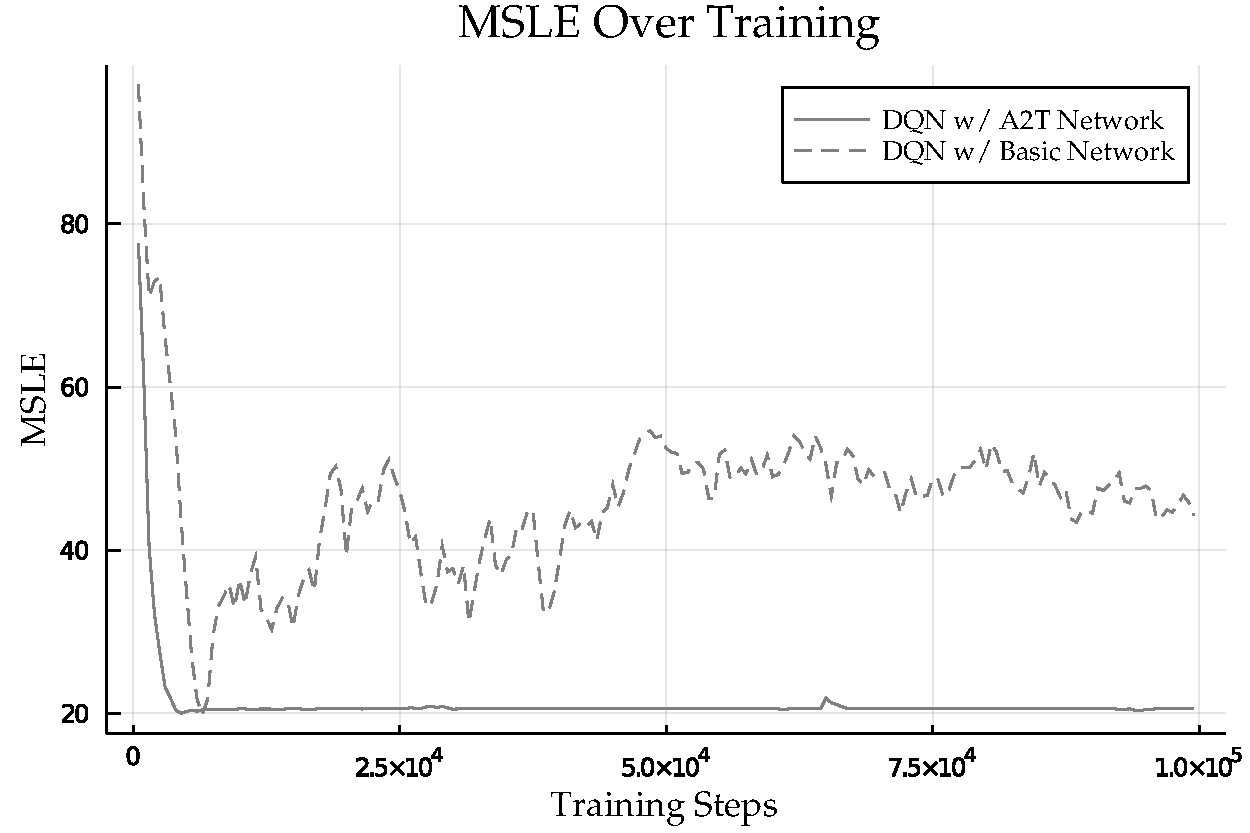
\includegraphics[width=\textwidth]{figures/scene_decomposition/training_comparison.pdf}
        \caption{Training comparison between A2T and basic network.}
        \label{fig:ch5_adv_gridworld_training}
\end{figure}


\section{T-Intersection Scenario}

\begin{table}
    \centering
    \caption{5-car Results}
    \label{tab:ch6_5car_results}
    \begin{tabular}{@{}lll@{}} 
        \toprule
        \textbf{Method} & \textbf{Failure Rate} & \textbf{Log Likelihood}\\
        \midrule
        Monte Carlo & \num{0.0} \pm \num{0.0} &  - \\
        Uniform Actions & \num{0.031} \pm \num{0.005} & \num{-173.01} \pm \num{42.925} \\
        Cross Entropy Method & \num{0.035} \pm \num{0.006} & \num{-82.672} \pm \num{7.342} \\
        DQN + A2T & \num{0.081} \pm \num{0.009} & \num{-19.938} \pm \num{7.317} \\
        \bottomrule
    \end{tabular}
\end{table}

\begin{figure}
        \centering
        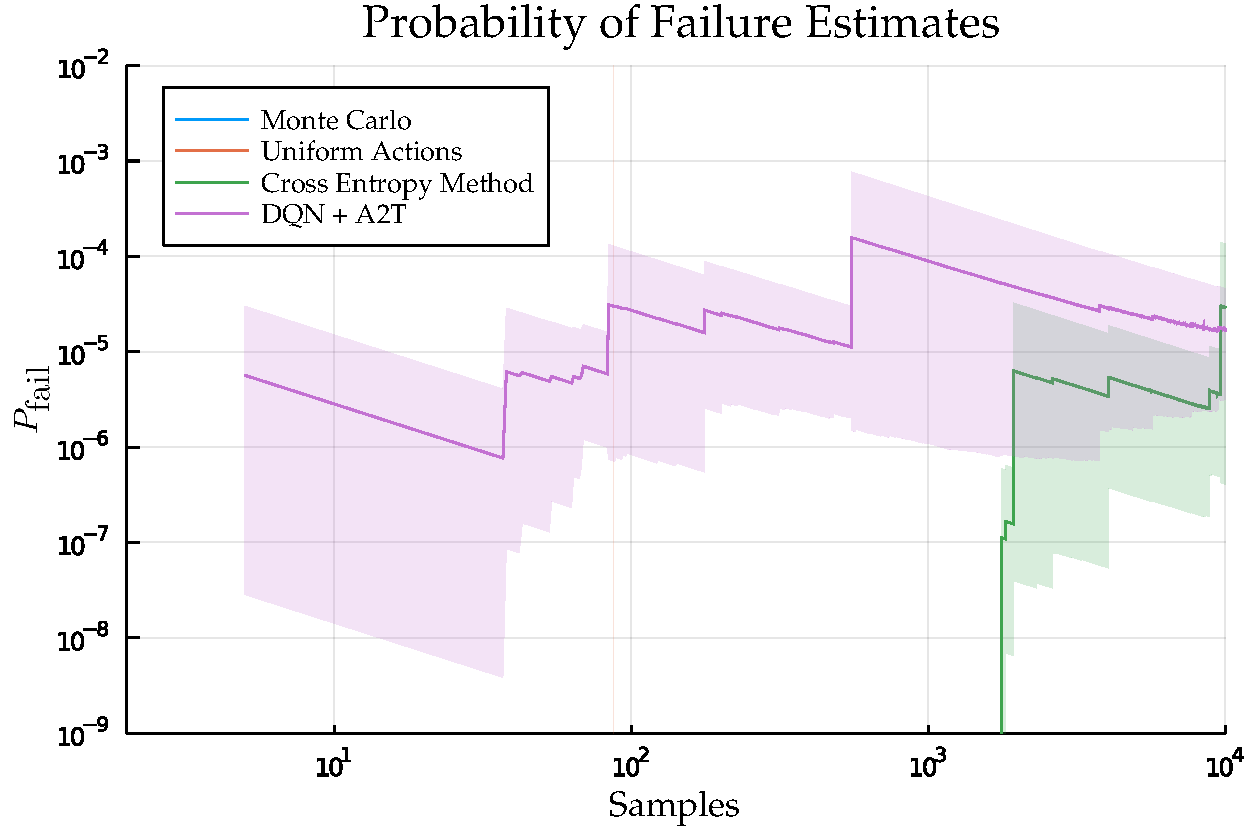
\includegraphics[width=\textwidth]{figures/scene_decomposition/pfail_5car.pdf}
        \caption{Comparison of techniques for $P_{\rm fail}$ estimation for the 5-car T-intersection scenario.}
        \label{fig:ch5_5car_pfail_estimation}
\end{figure}

\begin{figure}
    \centering
   \begin{subfigure}[t]{0.7\textwidth}
        \centering
        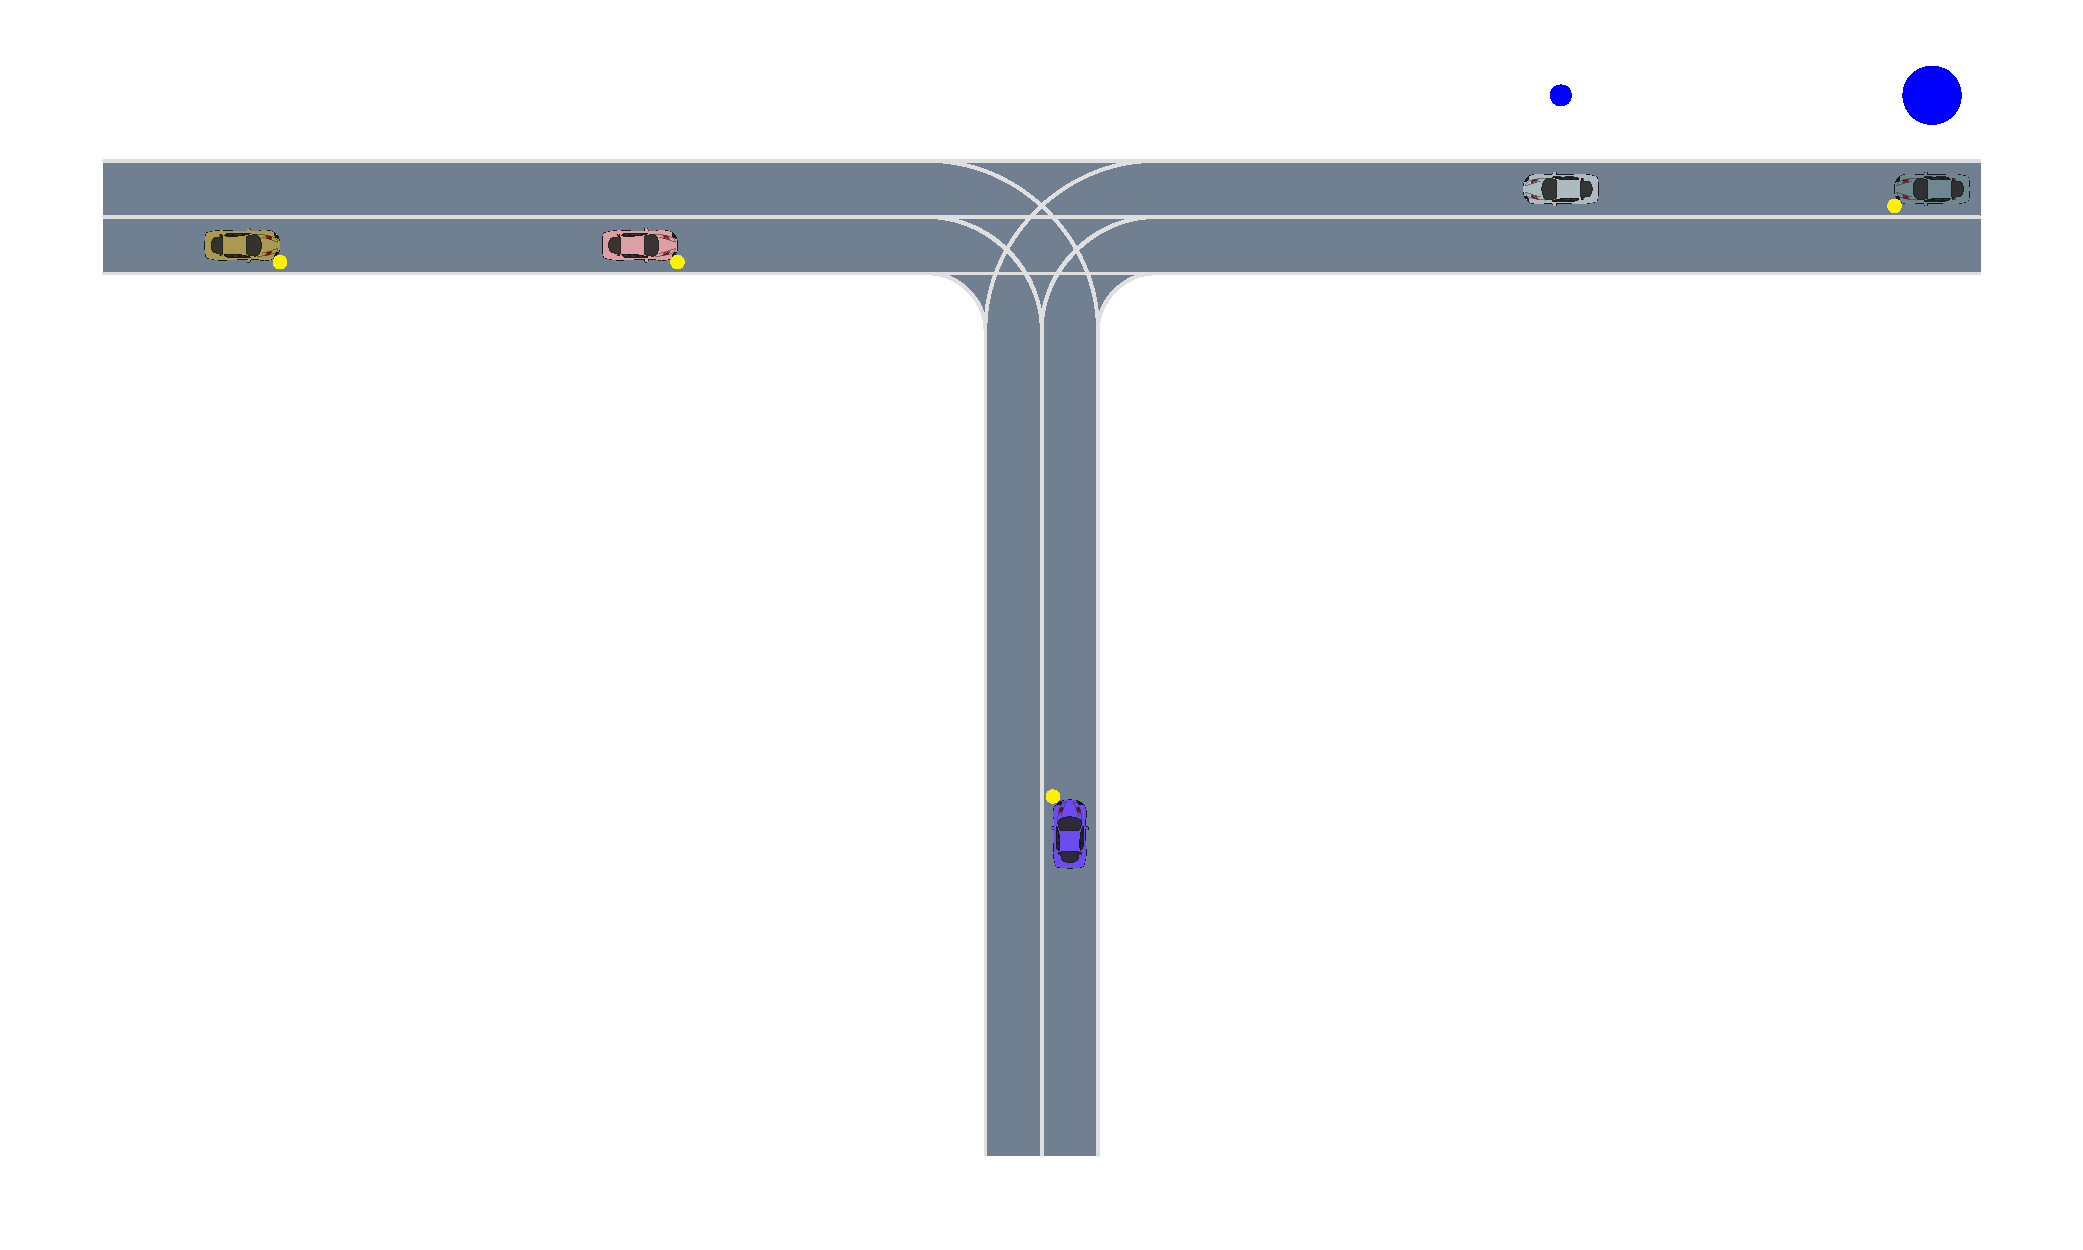
\includegraphics[width=\textwidth, trim={2cm 5cm 1cm 0},clip]{figures/scene_decomposition/f1_1.pdf}
    \end{subfigure}
    \begin{subfigure}[t]{0.7\textwidth}
        \centering
        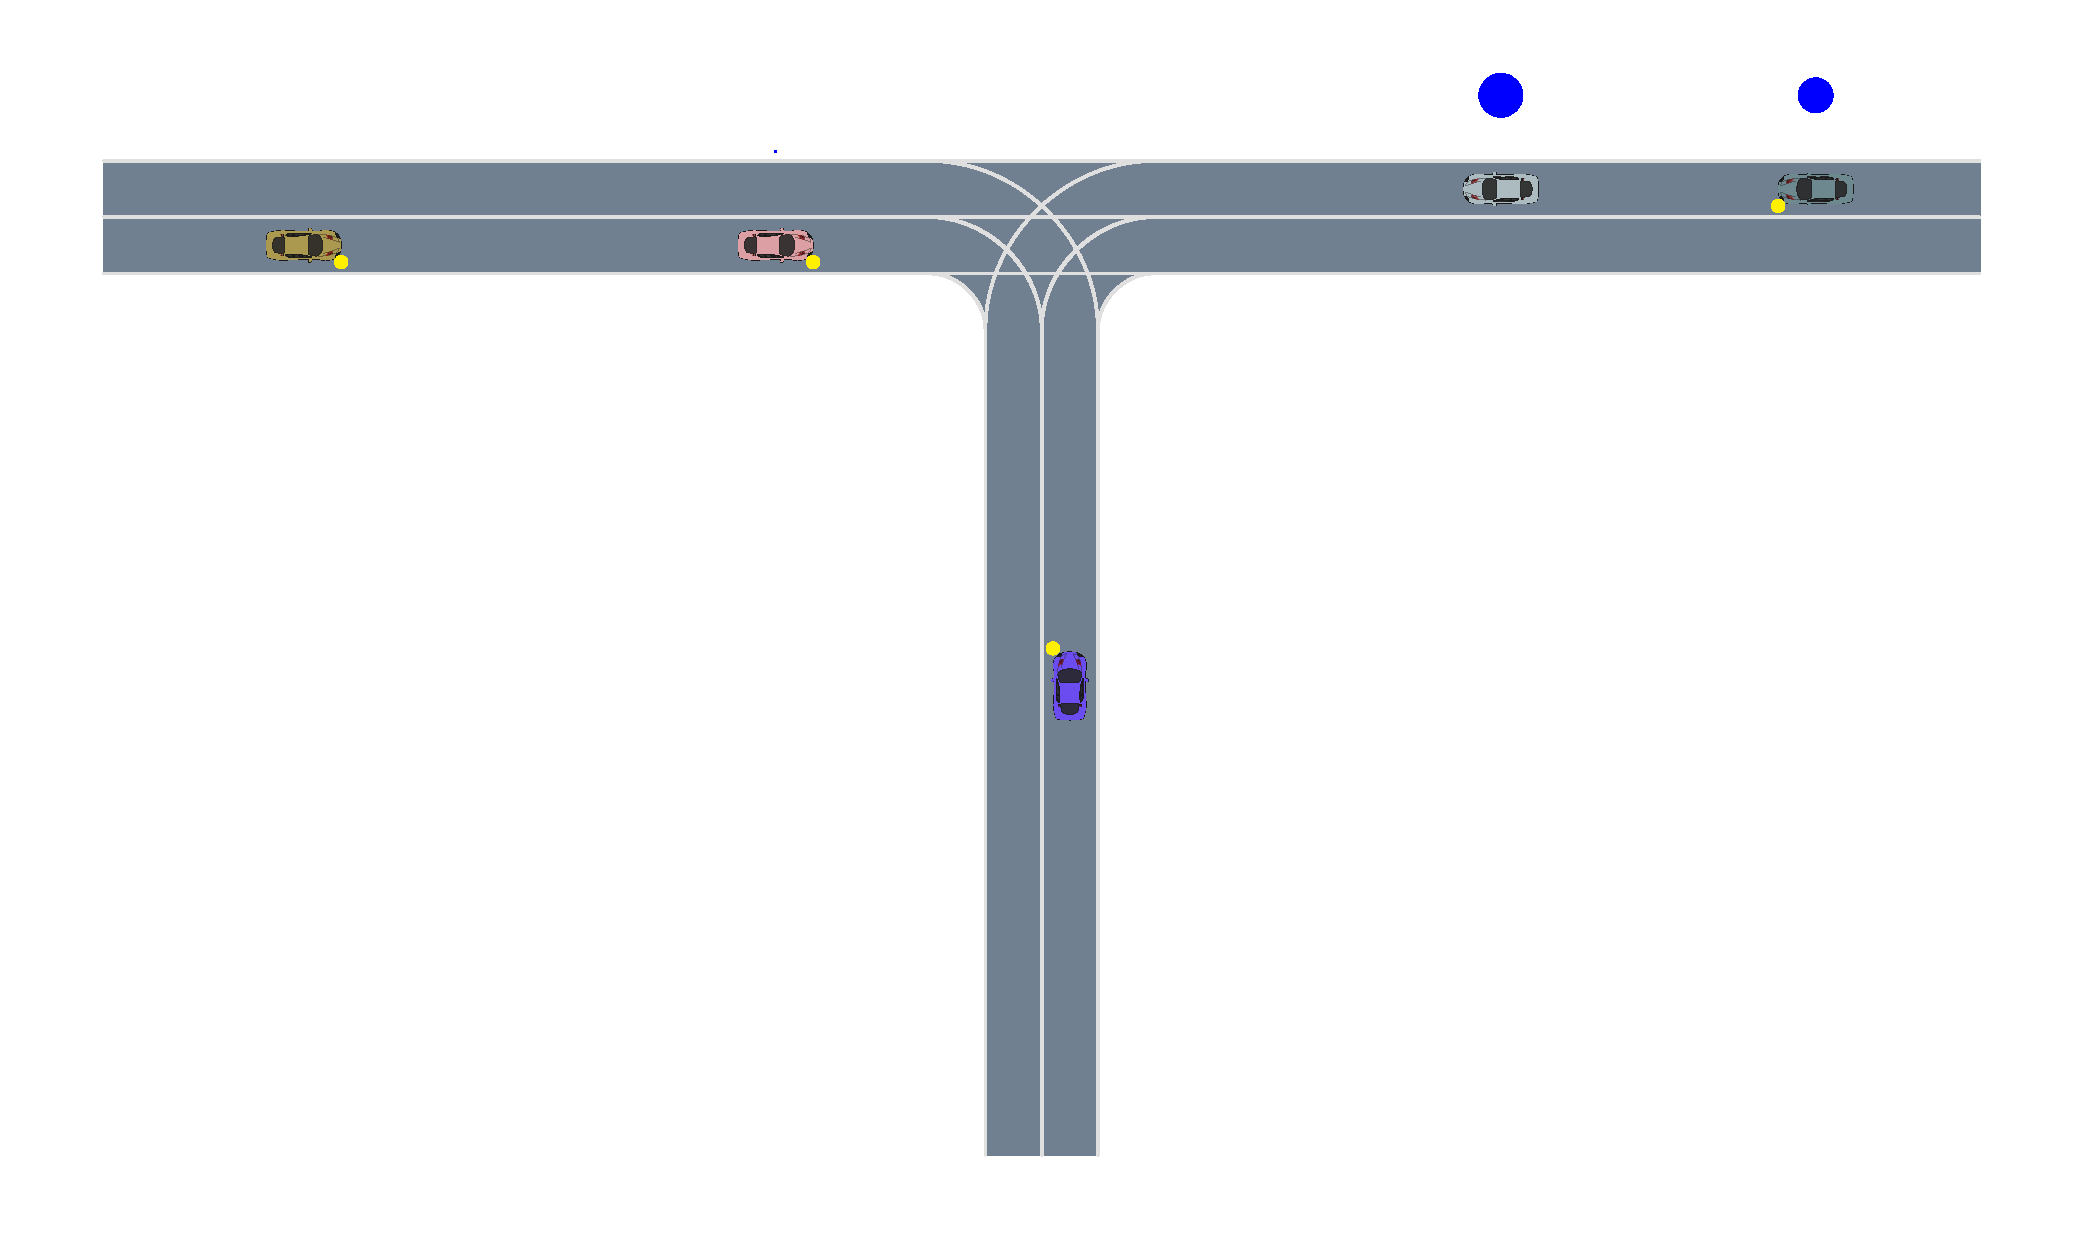
\includegraphics[width=\textwidth, trim={2cm 5cm 1cm 0},clip]{figures/scene_decomposition/f1_4.pdf}
    \end{subfigure}
    \begin{subfigure}[t]{0.7\textwidth}
    \centering
    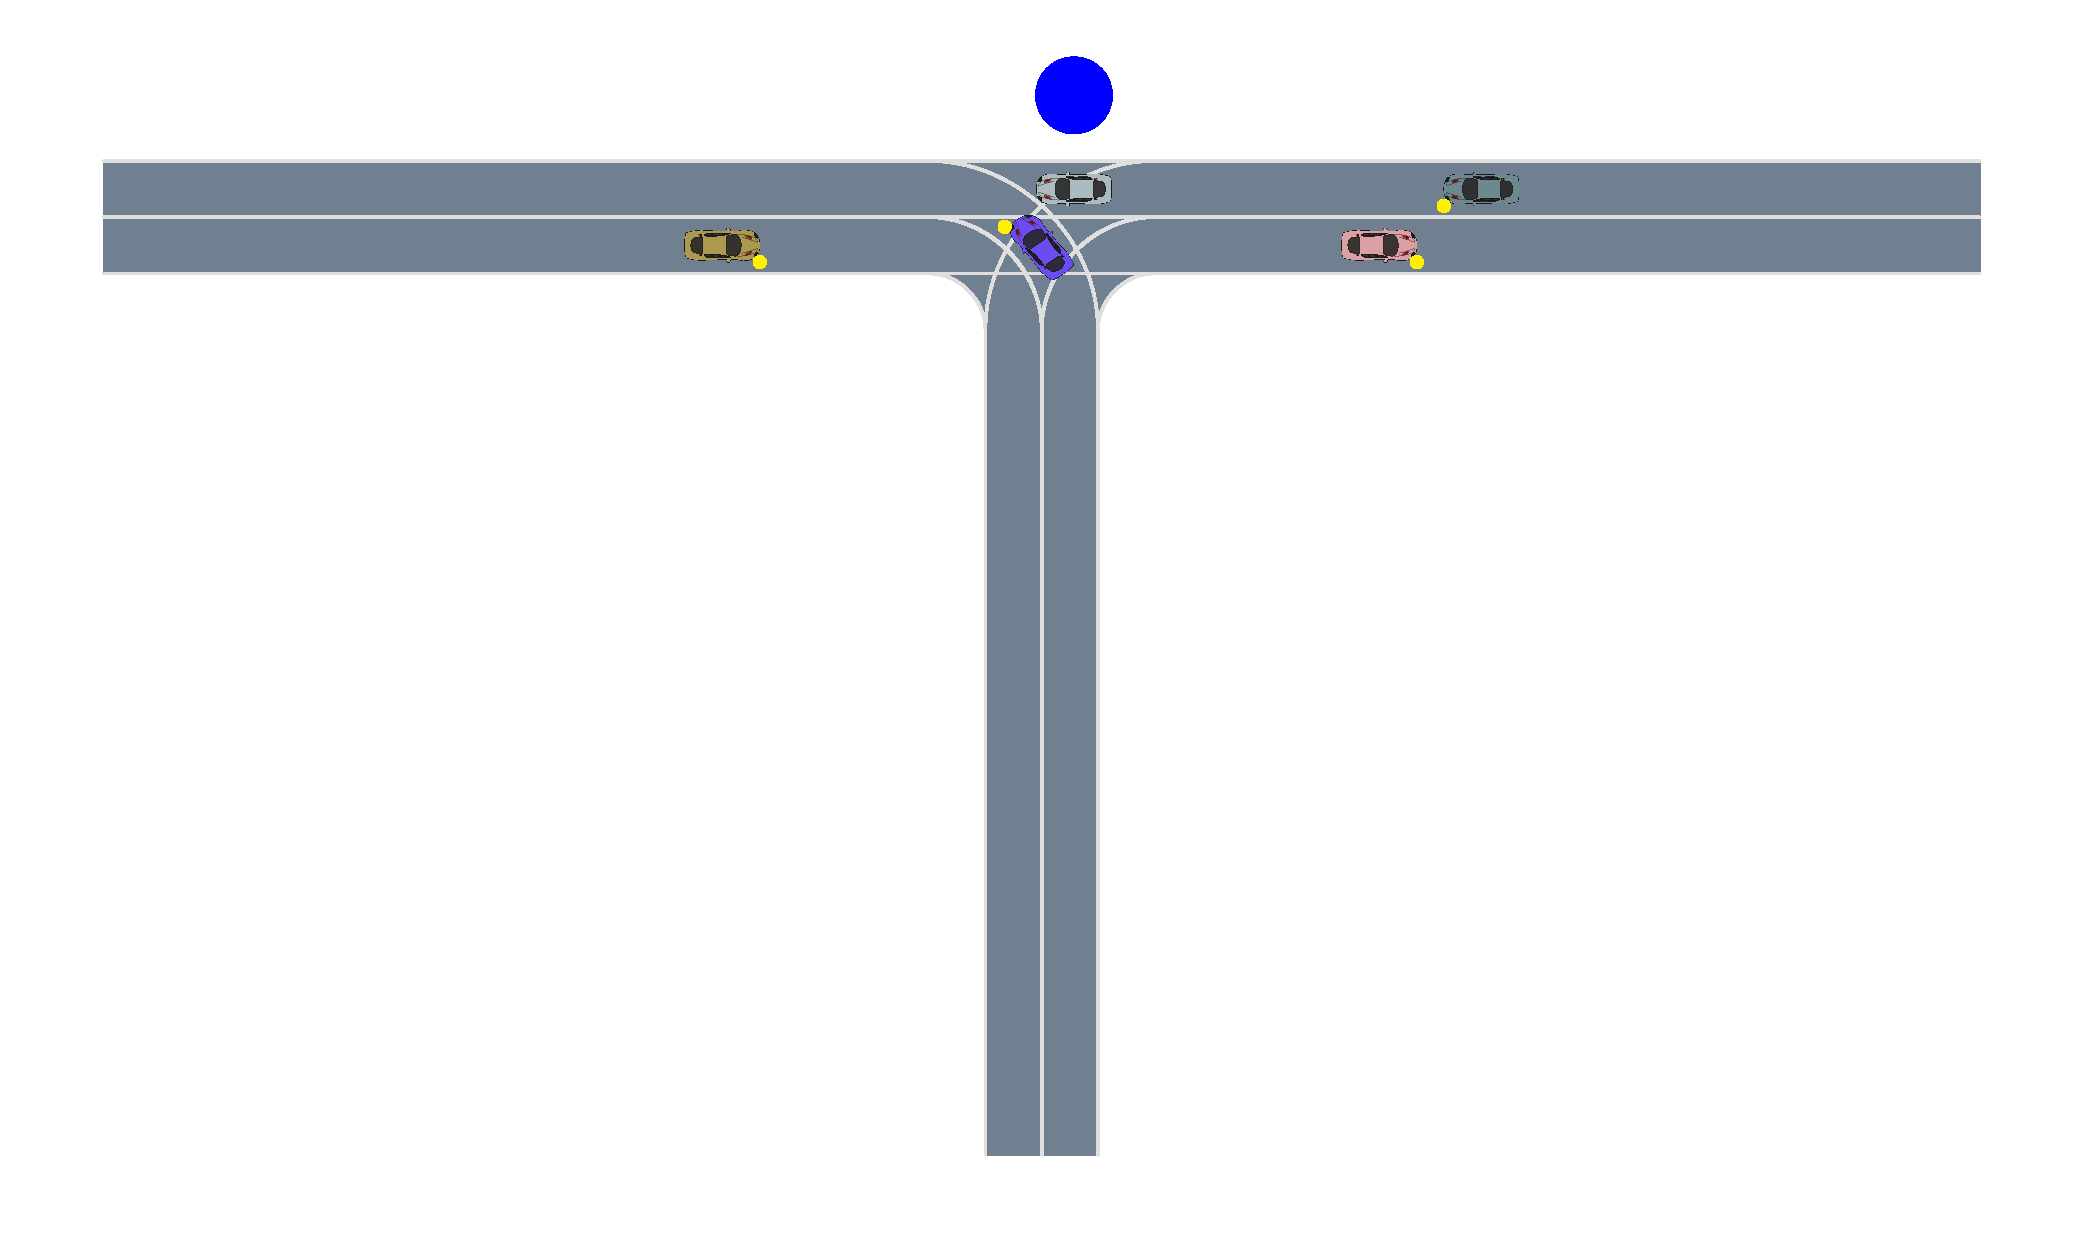
\includegraphics[width=\textwidth, trim={2cm 5cm 1cm 0},clip]{figures/scene_decomposition/f1_18.pdf}
\end{subfigure}
    \caption{Collision in 5-car scenario at timesteps $t=[1,4,18]$}
    \label{fig:two_car_collision}
    \vspace{-0.2in}
\end{figure}


\begin{figure}
    \centering
   \begin{subfigure}[t]{0.7\textwidth}
        \centering
        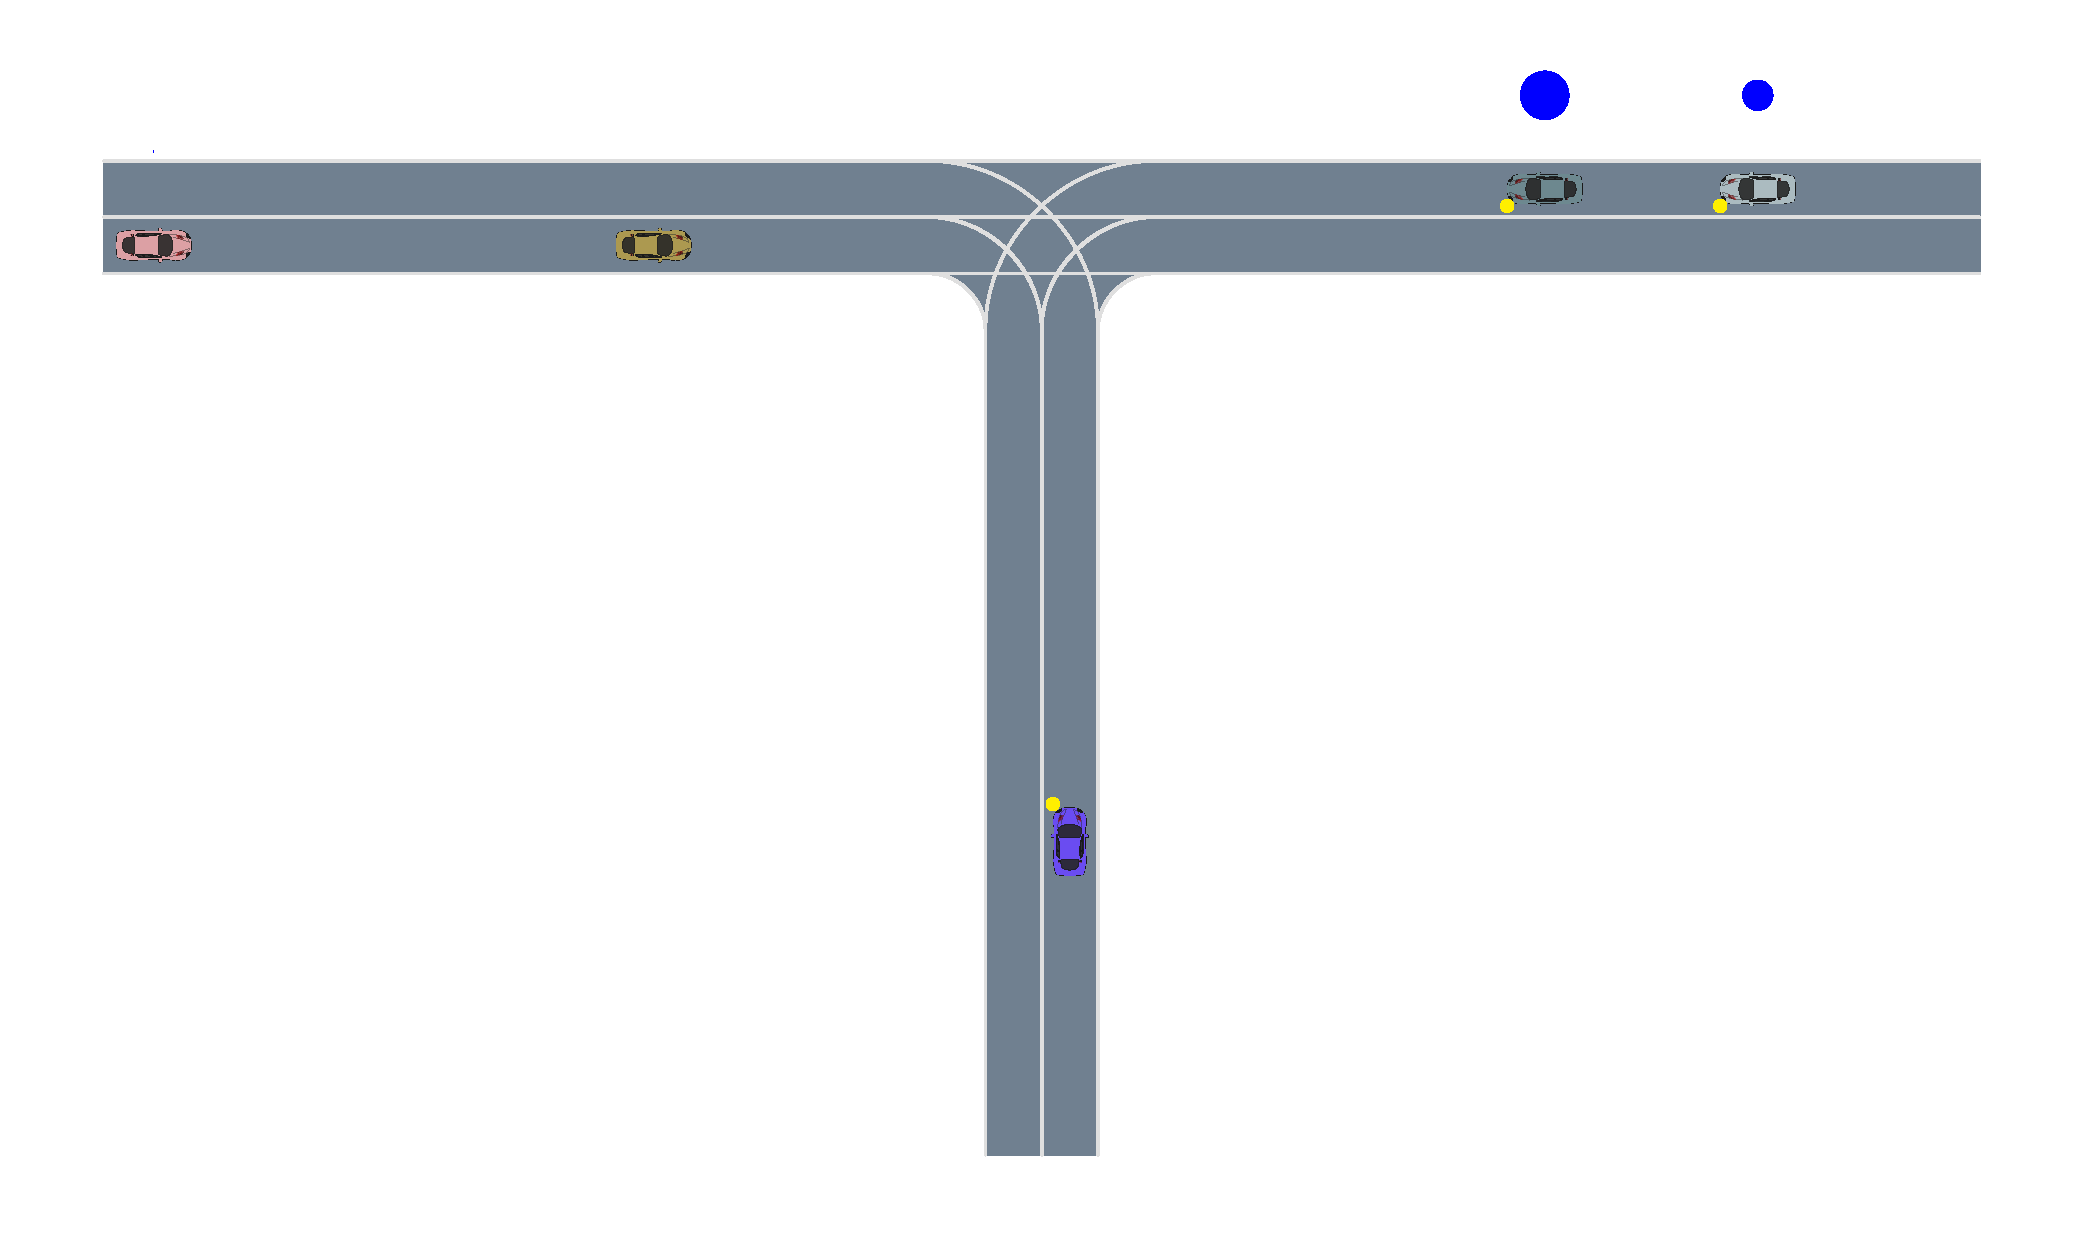
\includegraphics[width=\textwidth, trim={2cm 5cm 1cm 0},clip]{figures/scene_decomposition/f2_1.pdf}
    \end{subfigure}
    \begin{subfigure}[t]{0.7\textwidth}
        \centering
        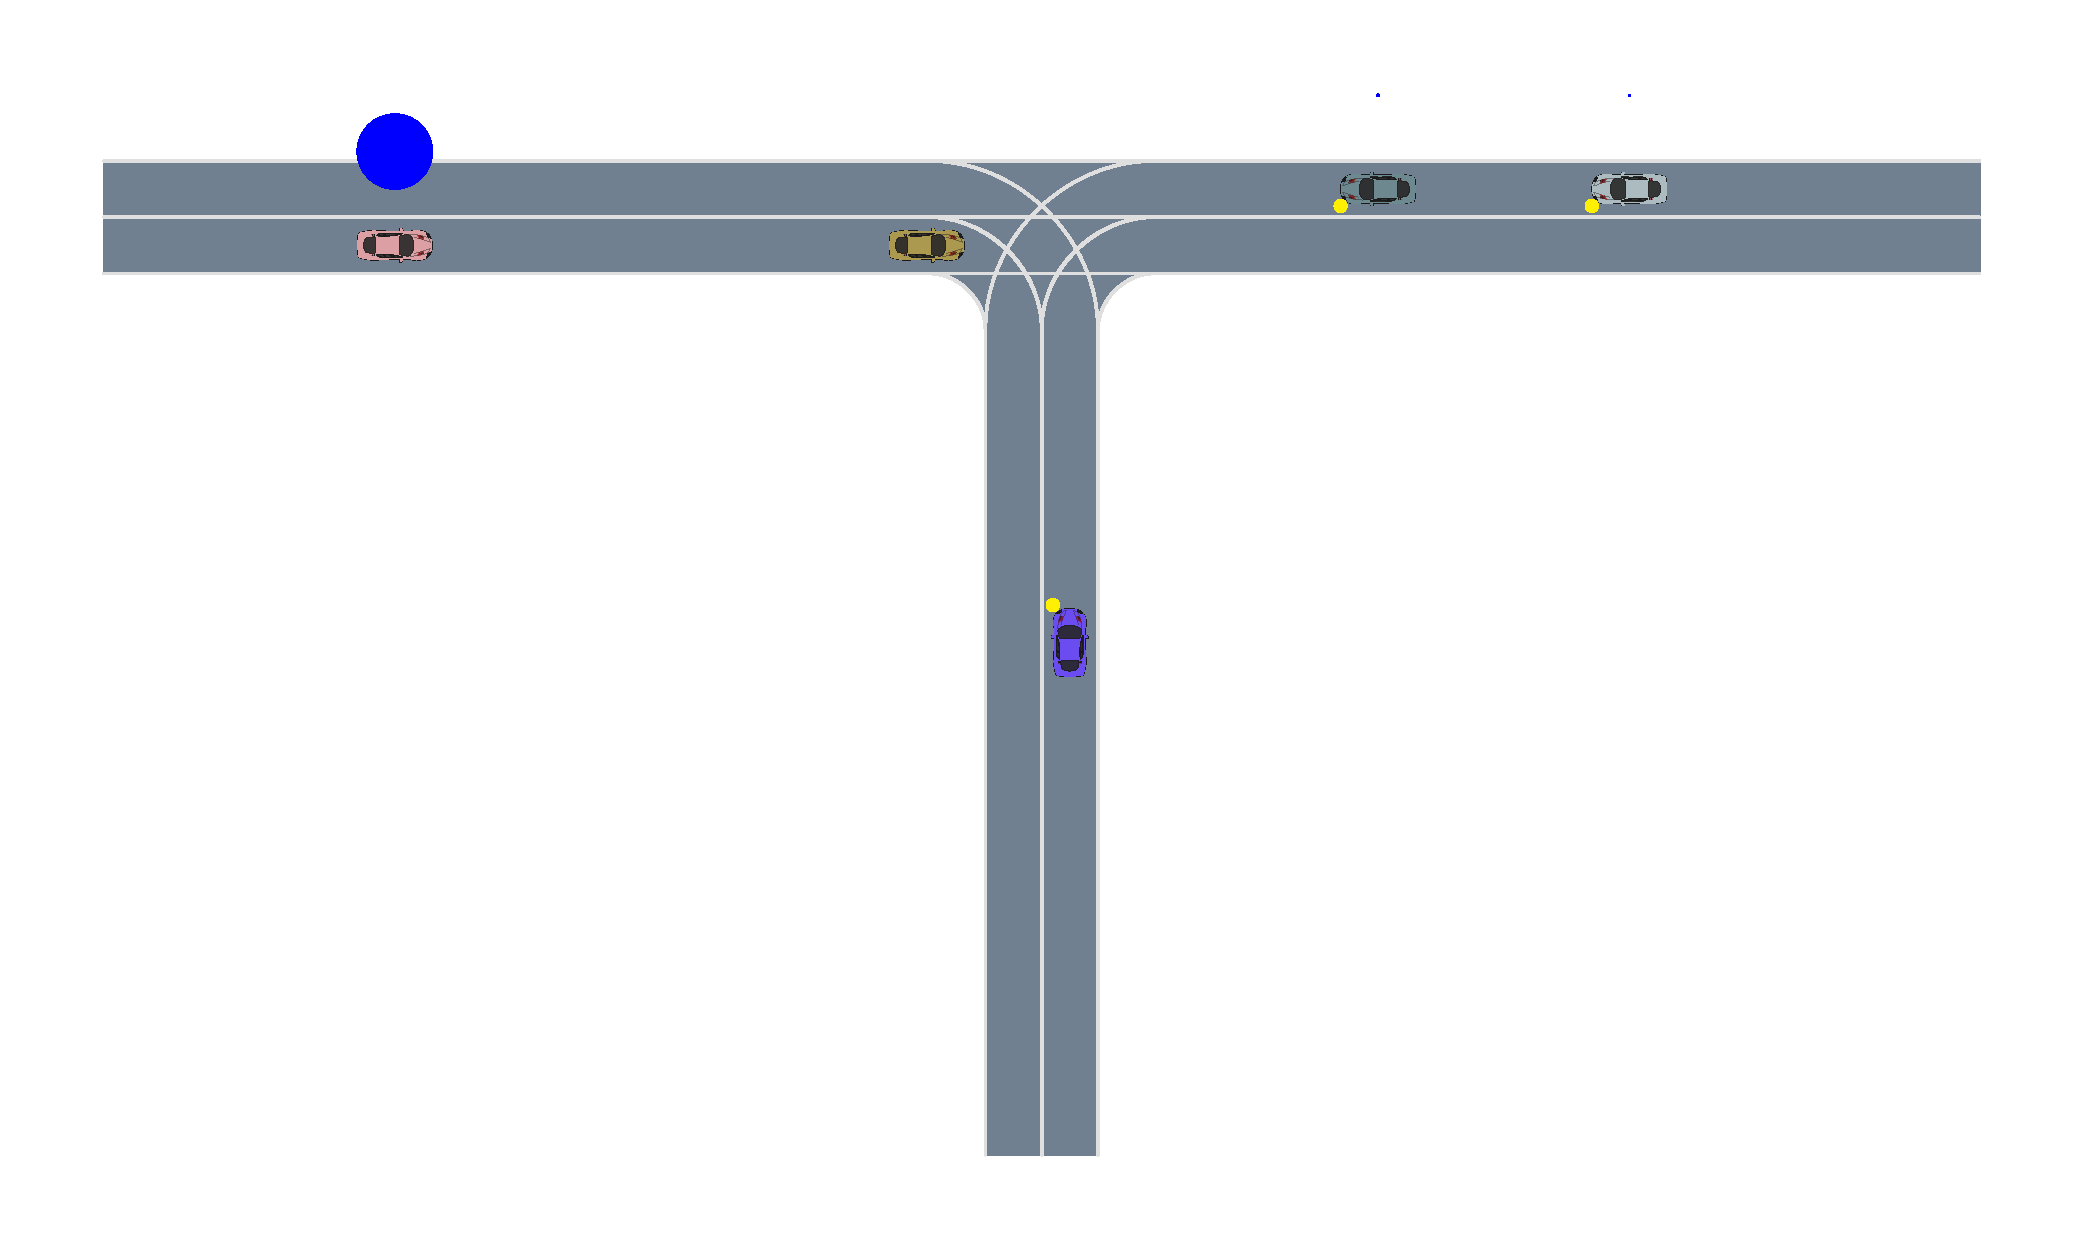
\includegraphics[width=\textwidth, trim={2cm 5cm 1cm 0},clip]{figures/scene_decomposition/f2_8.pdf}
    \end{subfigure}
    \begin{subfigure}[t]{0.7\textwidth}
    \centering
    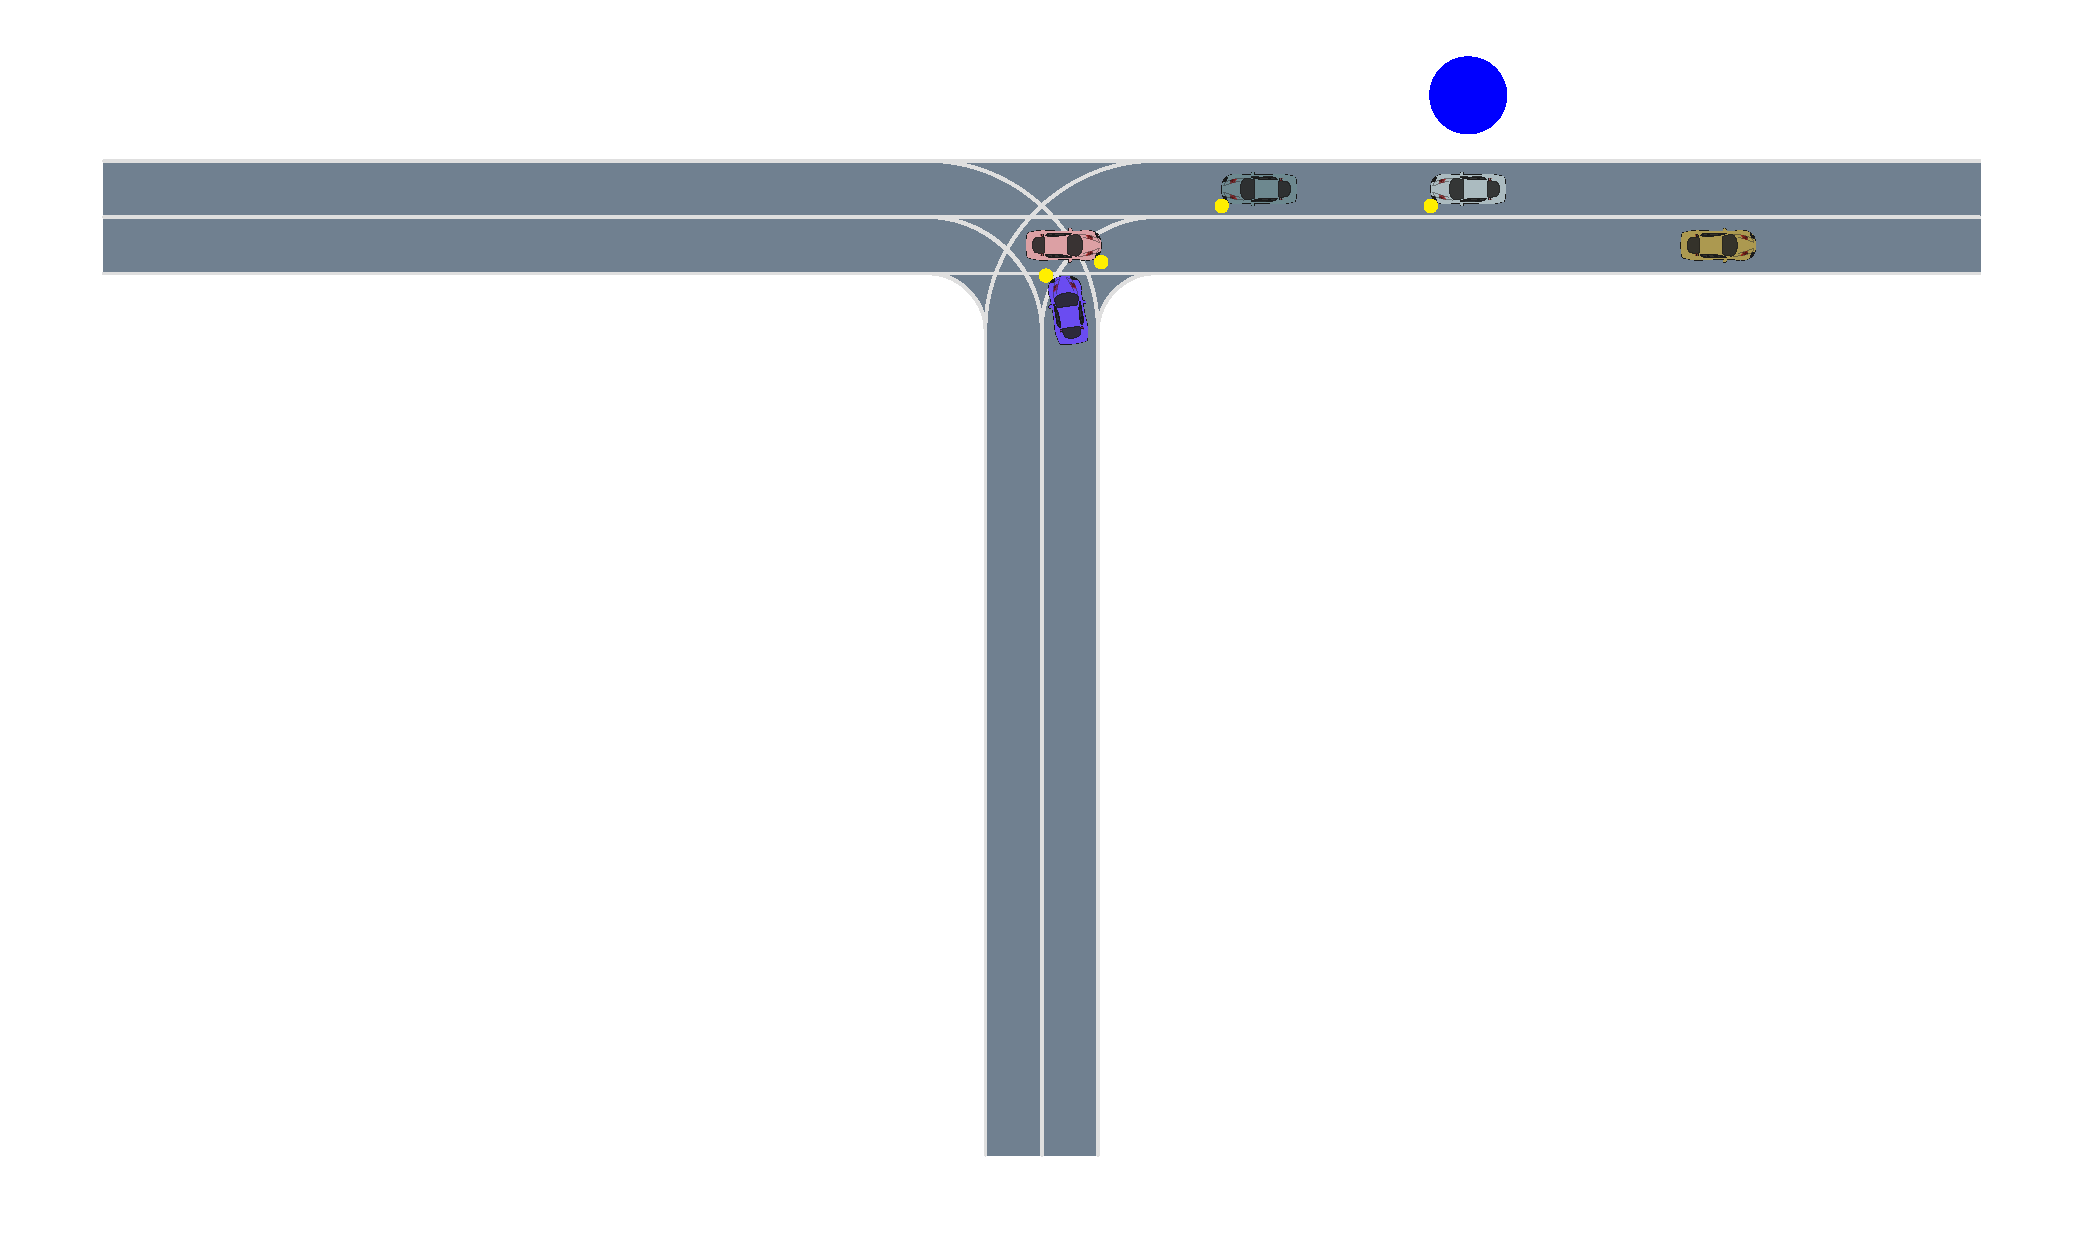
\includegraphics[width=\textwidth, trim={2cm 5cm 1cm 0},clip]{figures/scene_decomposition/f2_27.pdf}
\end{subfigure}
    \caption{Collision in 5-car scenario at timesteps $t=[1,8,27]$}
    \label{fig:two_car_collision}
    \vspace{-0.2in}
\end{figure}


\section{Discussion}